\newpage
\section{Die Messwerte}
\begin{table}[H]
    \centering
    %\caption{Die Messwerte}
    \label{tab:messung}
    \begin{tabular}{ S [table-format=2.0] S [table-format=2.1] S[table-format=2.2] S S[table-format=2.1] S [table-format=3.0] }
        \toprule
        {$t \mathbin{/} \si{\minute}$} & {$T_1 \mathbin{/} \si{\celsius}$} & {${p^{*}}_1 \mathbin{/} \si{\bar}$} & 
        {$T_2 \mathbin{/} \si{\celsius}$} & {${p^{*}}_2 \mathbin{/} \si{\bar}$} & {$\symup{N} \mathbin{/} \si{\watt}$}\\
        \midrule
        0	& 21.7&	4.0 &	21.7  &  4.1 &   120\\
        0	& 21.7&	4.0 &	21.7  &  4.1&    120\\
        0	& 21.7&	4.0 &	21.7  &  4.1 &   120\\
        3 &	 25.3&	6.0 &	21.5&	3.5&	   120\\
        4 &	 26.4&	6.0 &	20.8&	3.5	&   120\\
        5 &	 27.5&	6.0 &	20.1&	3.4	&   120\\
        6 &	 28.8&	6.5 &	19.2&	3.3	 &  120\\
        7 &	 29.7&	6.5 &	18.5&	3.2	 &  120\\
        8 &	 30.9&	7.0 &	17.7&	3.2	 &  120\\
        9 	& 31.9&	7.0 &	16.9&	3.0	 &  120\\
        10	 &32.9&	7.0 &	16.2&	3.0	 &  120\\
        11	& 33.9&	7.5 &	15.5&	2.9  &   120\\
        12	& 34.8&	7.5 &	14.9&	2.8  &  120\\
        13	& 35.7&	8.0 &	14.2&	2.8 &	120\\
        14	 &36.7&	8.0 &	13.6&	2.7	  &  120\\
        15&	 37.6&	8.0 &	13.0&	2.6	 &   120\\
        16&	 38.4&	8.5 &	12.4&	2.6 &	120\\
        17&	 39.2& 8.5 &	11.7&	2.6	&    120\\
        18&	 40.0&	9.0 &	11.3&	2.5  &   120\\
        19&	 40.7&	9.0 &	10.9&	2.5	 &   120\\
        20&	 41.4&	9.0 &	10.4&	2.4	 &   120\\
        21&	 42.2&	9.0 &	9.9	 &   2.4	 &   120\\
        22&	 42.9&	9.5 &	9.5	&    2.4	 &   120\\
        23&	 43.6&	9.5 &	9.1	&    2.4	 &   120\\
        24&	 44.3&	10.0&	8.7&    2.4	&    120\\
        25&	 44.9&	10.0&	8.3	&    2.4	 &   120\\
        26&	 45.5&	10.0&	8.0&	    2.3	 &   120\\
        27&	 46.1&	10.0&	7.7	&    2.2	 &   122\\
        28&	 46.7&	10.5&	7.4&	    2.2	 &   122\\
        29&	 47.3&	10.5&	7.1&	    2.2	 &   122\\
        30&	 47.8	&10.75&	6.8	&    2.2	 &   122\\
        31&	 48.4&	11.0&	5.6	 &   2.2	&    122\\
        32&	 48.9&	11.0&	4.3	&    2.2	 &   122\\
        33&	 49.4&	11.0&	3.4	&    2.2	 &   122\\
        34&	 49.9&	11.0&	3.0	&    2.2	&    122\\
        35&	 50.3&	11.0&	2.9	&    2.2	 &   122\\
        \bottomrule
        %\multicolumn{6}{c}{$\text{Eine Tabelle der Messwerte,}$}
        %\multicolumn{6}{c}{$\text{wobei die Temperaturen mit einem Fehler von  $\increment T = \SI{0.1}{\celsius}$ behaftet sind.}$}
    \end{tabular}
\caption{Eine Tabelle der Messwerte, wobei die Temperaturen mit einem Fehler von  $\increment T = \SI{0.1}{\celsius}$ behaftet sind.}
\end{table}



%5a)
\section{Gefitete Messwerte}
\subsection{Plot der Messwerte und Funktionen}
\begin{figure}
    \centering
    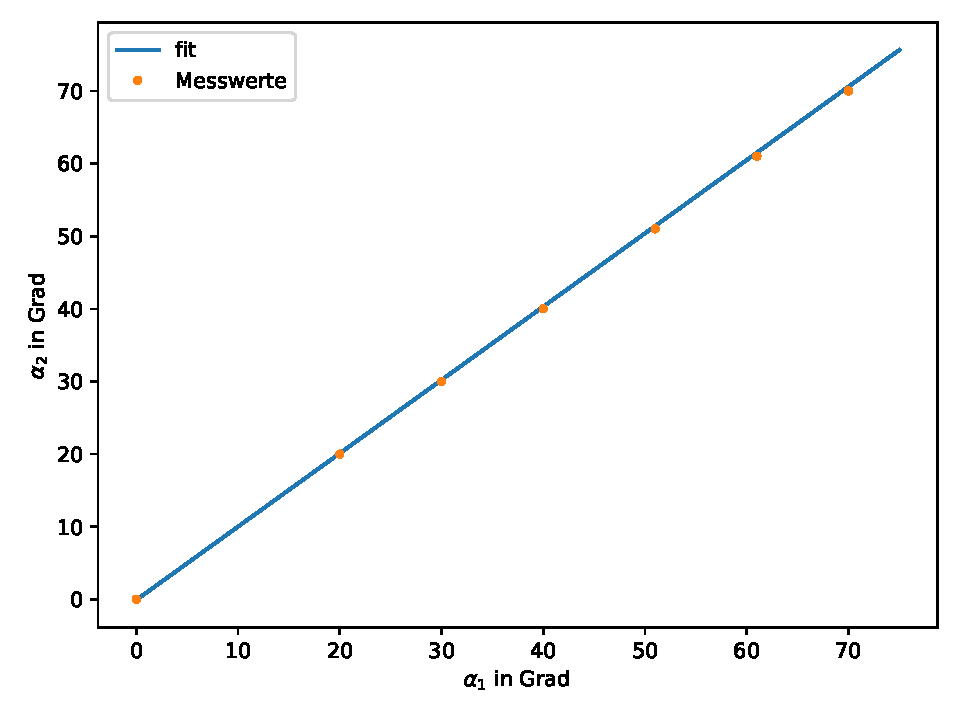
\includegraphics[width=\textwidth]{build/plot1.pdf}
    \caption{Ein Plot der Messwerte inklusive der gefiteten Funktionen.}
\end{figure}


%5b)
\subsection{Fit-Funktionen}
Dies sind die Fit-Funktionen auf die Messwerte. Dabei ist der Fit auf $T_1$ die Funktion $F(t)$ und der auf $T_2$ ist die Funktion $G(t)$.
\begin{align}
    F(t) &=A \cdot t^2+B \cdot t+ C \\
    G(t) &= \frac{D}{1+E \cdot t^{F}}\\
    &\begin{aligned}
        A &=0.00000322 & B&=0.02027984 & C&=21.82008061 \\
        D &=21.58061064 & E&= 0.00000095& F&=1.97775836 
    \end{aligned}\\
    F(t) &=0.00000322t^2+0.02027984t+21.82008061 \\
    G(t) &= \frac{21.58061064}{1+0.00000095t^{1.97775836}}
\end{align}
\\

%5c)
\section{Differentialquotienten der Temperaturen}
Im folgenden werden die Differentialquotienten der Temperaturen in verschiedenen Stellen berechnet.
Da die Fit Funktionen eine angemessene Abbildung der Messwerte darstellen berechnen wir die Quotienten über das bilden der Ableitung der Fits $F(t)$ und $G(t)$ 
und ihrer anschließenden Punktweisen Auswertung.
Als Punkte wurden hierbei 7er Schritte gewählt, da man daurch regelmäßige Abstände über den Definitonsbereich hat und einen breiten Bereich des selben abdeckt.


\begin{align}
    \frac{\partial F(t)}{\partial t} &=2At*B & \frac{\partial G(t)}{\partial t} &= \frac{-D \cdot F\cdot E \cdot t^{F-1}}{(1+E\cdot t^{F})^{2}}\\ 
\end{align}

\begin{table}[H]
    \centering
    \label{tab:Diff}
    \begin{tabular}{S S [table-format=1.4] S [table-format=2.4]}
        \toprule
        {Zeit [min]} & { $\frac{\partial F(t)}{\partial t}$ } & { $\frac{\partial G(t)}{\partial t}$ }  \\
        \midrule
        7	&0.0202 &-0.0147\\
        14	&0.0202 &-0.0139\\
        21	&0.0201 &-0.0134\\
        28	&0.0201 &-0.0131\\
        \bottomrule      
    \end{tabular}
\caption {Berechnete Werte für $v_\text{ideal}$ und $v_\text{real} $ gerundet auf die fünfte Nachkommastelle.}
\end{table}

%5d)
\section{Güteziffern}
Anschließend werden die idealen und realen Güteziffern der Wärmepumpe aus den zuvor berechneten Werten und 
den Formeln \eqref{eqn:videal} und \eqref{eqn:vreal}  bestimmt. 
Dabei werden für die Temperaturwerte immer für verschiedene Zeiten die korrespondierenden Messwerte genutzt.

\begin{equation}
    v_\text{ideal}= \frac{Q_1}{A} = \frac{T_1}{T_1-T_2}
    \label{eqn:videal}
\end{equation}

\begin{equation}
    v_\text{real}= \frac{\increment{Q_1}}{\increment t \cdot \symup{N} }
    \label{eqn:vreal}
\end{equation}

\begin{equation}
    \frac{\increment Q_1}{\increment t} = \left(m_1 c_w + m_k c_k \right)\frac{\increment T_1}{\increment t}
    \label{eqn:delQ}
\end{equation}\\

Für die reale Wärmepumpe gilt $v_\text{real} < v_\text{ideal}$.\\

Der Wert für die reale Wärmepumpe lässt sich dann bestimmen, 
in dem man für die Wärmekapazität der Kupferschlange $m_k c_k =\SI{750}{\joule\per\kelvin}$,
für die Masse des Wassers $m_1=\SI{4}{\kilo\gram}$ und für die spezifische Wärmekapazität 
des Wassers $c_w=\SI{4.183}{\kilo\joule\per\kilo\gram\per\kelvin}$ nimmt.
Anshließend setzt man dann \eqref{eqn:delQ} in \eqref{eqn:vreal} ein. 
Es ergibt sich dann also aus den zuvor bestimmten Werten;

\begin{table}[H]
    \centering
    \label{tab:vreal}
    \begin{tabular}{ S [table-format=2.0] S [table-format=1.5] S [table-format=1.5] }
        \toprule
        {$t \mathbin{/} \si{\minute}$} & { $v_\text{ideal}$} & {$v_\text{real} $} \\
        \midrule
        7	&3 &0.12929\\
        14	&1.66047 &0.12900\\
        21	&1.33548 &0.12871\\
        28	&1.20052 &0.12632\\
        \bottomrule
        \\
    \end{tabular}
\caption {Berechnete Werte für $v_\text{ideal}$ und $v_\text{real} $ gerundet auf die fünfte Nachkommastelle.}
\end{table}












%\begin{align*}
%\intertext{Es ergibt sich dann also;}
%\end{align*}







